\documentclass[a4paper, 12pt]{report}

\oddsidemargin 0.5in \textwidth 5.75in \textheight 8.25in
\renewcommand{\baselinestretch}{1}

\usepackage[latin1]{inputenc}
\usepackage{graphicx}
\usepackage{alltt}
\usepackage{hyphenat}
\usepackage{xcolor}
\usepackage{appendix}
\usepackage{listings}
%\usepackage{biblatex}

\title{Assessing the impact of gene sequence clustering strategies in
determining microbe-
microbe interactions in environmental microbiome datasets}
\author{Priyansh Srivastava}

\begin{document}

\begin{titlepage}
\setlength{\topmargin}{-0.6in}

\begin{figure}[!h]
  \centering
  
\includegraphics[width=6cm]{logo.png}
\end{figure}
\vspace{1cm}

\begin{center}
{\LARGE \bigskip\textbf{Assessing the impact of gene sequence clustering strategies in determining microbe-
microbe interactions in environmental microbiome datasets}}

\vspace{1.25cm}
{\normalsize A thesis submitted \vspace{.5cm}\\ by \vspace{.5cm}\\
\vspace{1.25cm} Priyansh Srivastava \vspace{1.25cm} \\ to \vspace{.5cm} \\
The Discipline of Bioinformatics, \\ School of Mathematics, Statistics \& Applied Mathematics \\ National University \textit{of} Ireland, Galway \vspace{1cm} \\ in partial fulfilment of
the requirements for the degree of \\ \vspace{.5cm} M.Sc. in
Computational Genomics \vspace{1cm} \\ April 23rd 2020 \\
\vspace{1.25cm} Thesis Supervisor: Dr Alexandre De Menezes}

\end{center}
\end{titlepage}

%\maketitle

\begin{abstract}

TBC

\end{abstract}


\pagenumbering{roman} \setcounter{page}{2}
\tableofcontents
\newpage

\listoffigures
\listoftables

\chapter{Introduction}
\pagenumbering{arabic} \setcounter{page}{1}

\section{Overview}
Life on earth sprang from microscopic uni-celled organisms roughly around 4 billion years ago. Since then, these tiny life forms have been dwelling in every part of the earth. From extreme abiotic environments to complex life forms, microbial life is omnipresent. Prokaryotic microbes are the principal recyclers of the biosphere and form the largest reserve of nutrients \textcolor{green}{such as} phosphorus (P), Nitrogen (N) and Carbon (C) [1,2]. Essentially they are a vital constituent of nutrient cycles and food chains through which complex life forms are sustained. It has been evaluated that our microbiome size surpasses the total number of our cells [3,4]. Yet, genomic studies on these simple life forms are troublesome to perform because most of these microbes are difficult to culture in the labs and rarely exist in isolation [5]. Owing to these hurdles, even the studies conducted using microbial clonal cultures do not reflect the microbial community's actual biology and communal interactions [2]. However, with the \textcolor{green}{development} in next-generation sequencing (NGS) technology, scientists have succeeded in overcoming quite a few challenges in the field of microbial genomics. This branch of genomics which specifically elucidates the molecular study of those microscopic life forms that are hard to culture, has been assigned the term Metagenomics [6]. Metagenomic studies eliminate the need for clonal cultures and allow direct environmental sampling of the microbial communities (metagenome) [7]. This provides a highly descriptive assay illustrating a comprehensive view of both the microbial genome and biological interactions of the community [7].

\section{Impact of Genomics}
Generally, metagenomic procedures either employ 16s Ribosomal RNA (16s-rRNA) (for eukaryotes, it is 18s rRNA) sequencing methods or Whole Genome Shotgun (WGSS) sequencing methods. Both of these methodologies require trimming, error correction and reference database comparisons [8]. De-novo assemblies which do not require reference database comparisons are also exercised when the reference database is unavailable; however, they need more computational resources. 16s-rRNA genes are of tremendous significance as they hold the highly conserved genes and can be used to generate phylogenetic relations among microbial communities [8]. 16s-rRNA sequencing uses Polymerase Chain Reaction (PCR) to amplify the hypervariable segment (v1-V9) of prokaryotic 16s-rRNA, which generates amplicons that are then multiplexed, i.e. pooled together after applying molecular barcodes. This strategy is also called Amplicon sequencing. In fungal genomes, the Internal Transcribed Spacer (ITR) region is targeted; therefore,  it suffers from a high false-positive rate and host DNA interference [9]. Contrary to that, 16s-rRNA sequencing is affordable and offers a better taxonomic resolution at the genus and species level due to the availability of highly curated datasets. A 2019 study conducted by Gupta et al. also demonstrated that the 16s-rRNA provides more sensitive and comprehensive insights when compared to the traditional culture methods (TCMs). The results reflect that the 16s-rRNA identifies ~75\% unique elements, whereas the TCMs were only able to locate ~23\% bacterial elements [10]. 16s-rRNA sequencing either delivers Amplicon Sequence Variants (ASVs) or Operational Taxonomic Units (OTUs) depending upon the pipeline used for clustering. OTUs are the clusters of sequencing reads generated through a dissimilarity threshold filter. In contrast, the ASVs are exact sequences to a single nucleotide level offering a more acceptable resolution [11]. A more detailed comparison of OTUs and ASVs is discussed later in the review.

\section{Soil Ecology}
Soil ecology is one of the highly reshaped fields of soil microbiology by the addition of NGS technology. Microbial soil ecology studies how microbes interact; it was previously thought to be a dead area; however, after displacing TCMs with the WGSS/16s-rRNA methods, the area is revolutionised [12]. In the last decades, soil microbiologists have discovered a plethora of novel taxa (phyla, classes, genus) owing to metagenomics [12]. Soil metagenomics attempts to answer some of the requisite ecological questions like how microbial communities form? Or how communities communicate in space-time through signalling? Through international collaborations, soil microbiologists and bioinformaticians are also generating sophisticated datasets to help future scientists perform reference assemblies. In 2010 Earth Microbiome Project was announced which intends to collect and analyse the microbial community of the earth [13]. Similarly, in 2014 Brazillian Microbiome Project and China Soil Microbiome Initiative were announced, which have the related vision of exploring microbial communities [14,15]. Now that we have the tools to look at microbial life precisely, we can also implement system/network science principles to do a habitat-based examination of the microbial community. By utilising highly conserved 16s rRNA methods and adding molecular phylogeny of the population, we can understand biological interactions adequately [16]. One such approach is the study of co-occurrence networks. Co-occurrence networks can help interpret the effect of interspecies interactions like mutualism and parasitism [17]. Fundamentally, the interactions can be either positive or negative, influencing either aggregation or segregation. The positive interactions include cooperative processes like quorum sensing, whereas the antagonistic interactions include phenomenon like competition [18]. Microbial co-occurrences networks can illustrate the biological interactions well; however, in 2014, berry et al. demonstrated that these networks lose interpretability when habitat filtering (i.e. tolerance to local stress) becomes notable. Yet, Goberna et al. conducted a study by employing phylogenetic metrics in co-occurrence networks. They concluded that phylogenetic relatedness could help to explain ecologically essential patterns under the influence of habitat filtering [19]. However, the impact of OTUs and ASVs is still an uncharted territory.\newline \newline The current review addresses the crucial fundamentals of the metagenomic studies, featuring the 16s-rRNA sequencing method. The review further discusses the two widely used 16s-rRNA sequencing pipelines that produce different sequences tables, i.e. ASVs and OTUs. Lastly, a detailed study of microbial co-occurrence is discussed, accompanied by molecular phylogenetics. The review aims to reflect on the widely used pipelines with phylogenetic metrics and interpret ecological patterns from microbial co-occurrence networks.
\chapter{Metagenomics Essentials}
\pagenumbering{arabic} \setcounter{page}{4}

This section reviews the procedural steps involved in a typical metagenomics workflow. This section also covers the pre-requisites in metagenomics which one should contemplate before setting up an experiment.

\section{Sampling \& Quality Control}
Ideally, the obtained samples should be representative of the population from which they are pooled. Moreover, the sampling should be done blindly to reduce human biases. Also, pooled samples should carry high-quality nuclear material, which decreases the signal-to-noise ratio in the downstream analysis. If the target community is linked with a host organism, selective lysis must be conducted to reduce the host DNA interference \cite{ref11}. To plan the number of samples required, a refraction curve is often used \cite{ref11}. The rarefaction curve proposes abundance of existing species as function of inspected species [Figure \ref{fig:figure1}]. It is also desirable to look for pilot studies to determine the number of samples required from a particular habitat.

\begin{figure}
  \centering
  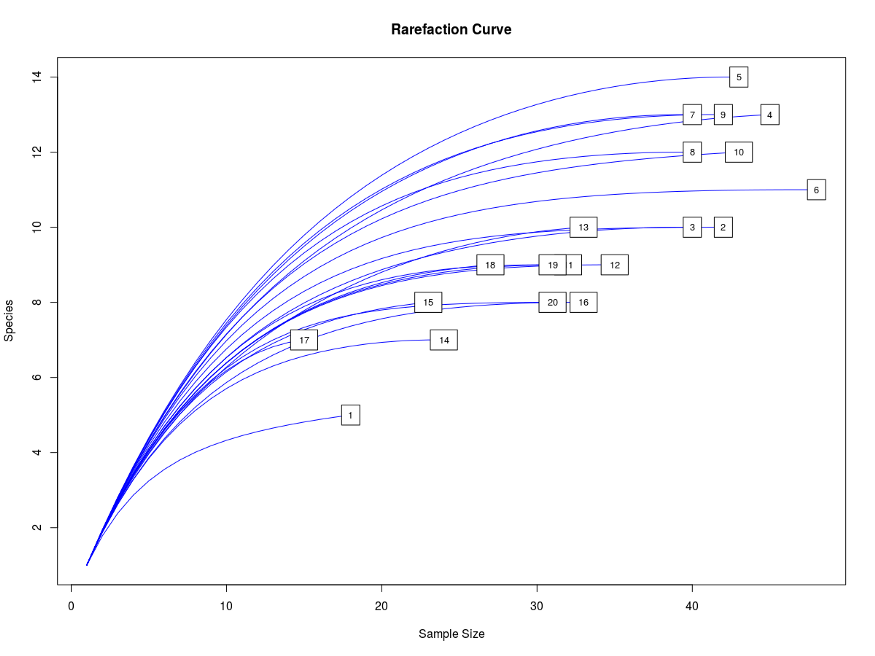
\includegraphics[width=9cm, height=5.5cm] {../figures/Figure1.png}
  \caption[Typical Rarefaction Curve]{Typical Rarefaction Curve displaying how many species are identified with prolonged sampling. If sampling is ample, curves should plateau as it becomes tougher to find new species, despite the increase in sampling. On the other hand, if the curves are steep, more sampling is required to infer ecological judgments \cite{ref11}}
  \label{fig:figure1}
\end{figure}

Once the samples are secured, they should be filtered to reduce the signal to noise ratio in downstream analysis. This can be achieved by either eliminating the noise (e.g. removing virome if studying bacteria) or collecting surplus signals (e.g. collection of high-quality samples) \cite{ref12}. Often it is hard to replicate metagenomic analysis as even the slightest deviation from the collection site appends variability to results. Therefore, precise documentation of the metadata is also vital to metagenomics; parameters like sampling date, time, depth, salinity, et cetera should be reported \cite{ref12}. A recent report from The Genomics Standards Consortium published a standard for reporting metagenomic metadata \cite{ref12}.

\section{Sequencing}
Over the years, second-generation sequencing methods have taken over the area of genomics [Figure \ref{fig:figure2}]. The Sanger Shotgun sequencing method (SS), the reasonable option of researchers in the past, has been displaced by PCR based methods, especially for smaller metagenomes. Despite being labour intensive and costly, the SS sequencing method is still preferred when dealing with specimens from low-diversity environments because it gives a comprehensive portrayal of genomes \cite{ref12}. Third-generation sequencing methods are gradually becoming the preference for metagenomics as they give long reads which aid in de-novo assemblies.

\begin{figure}
  \centering
  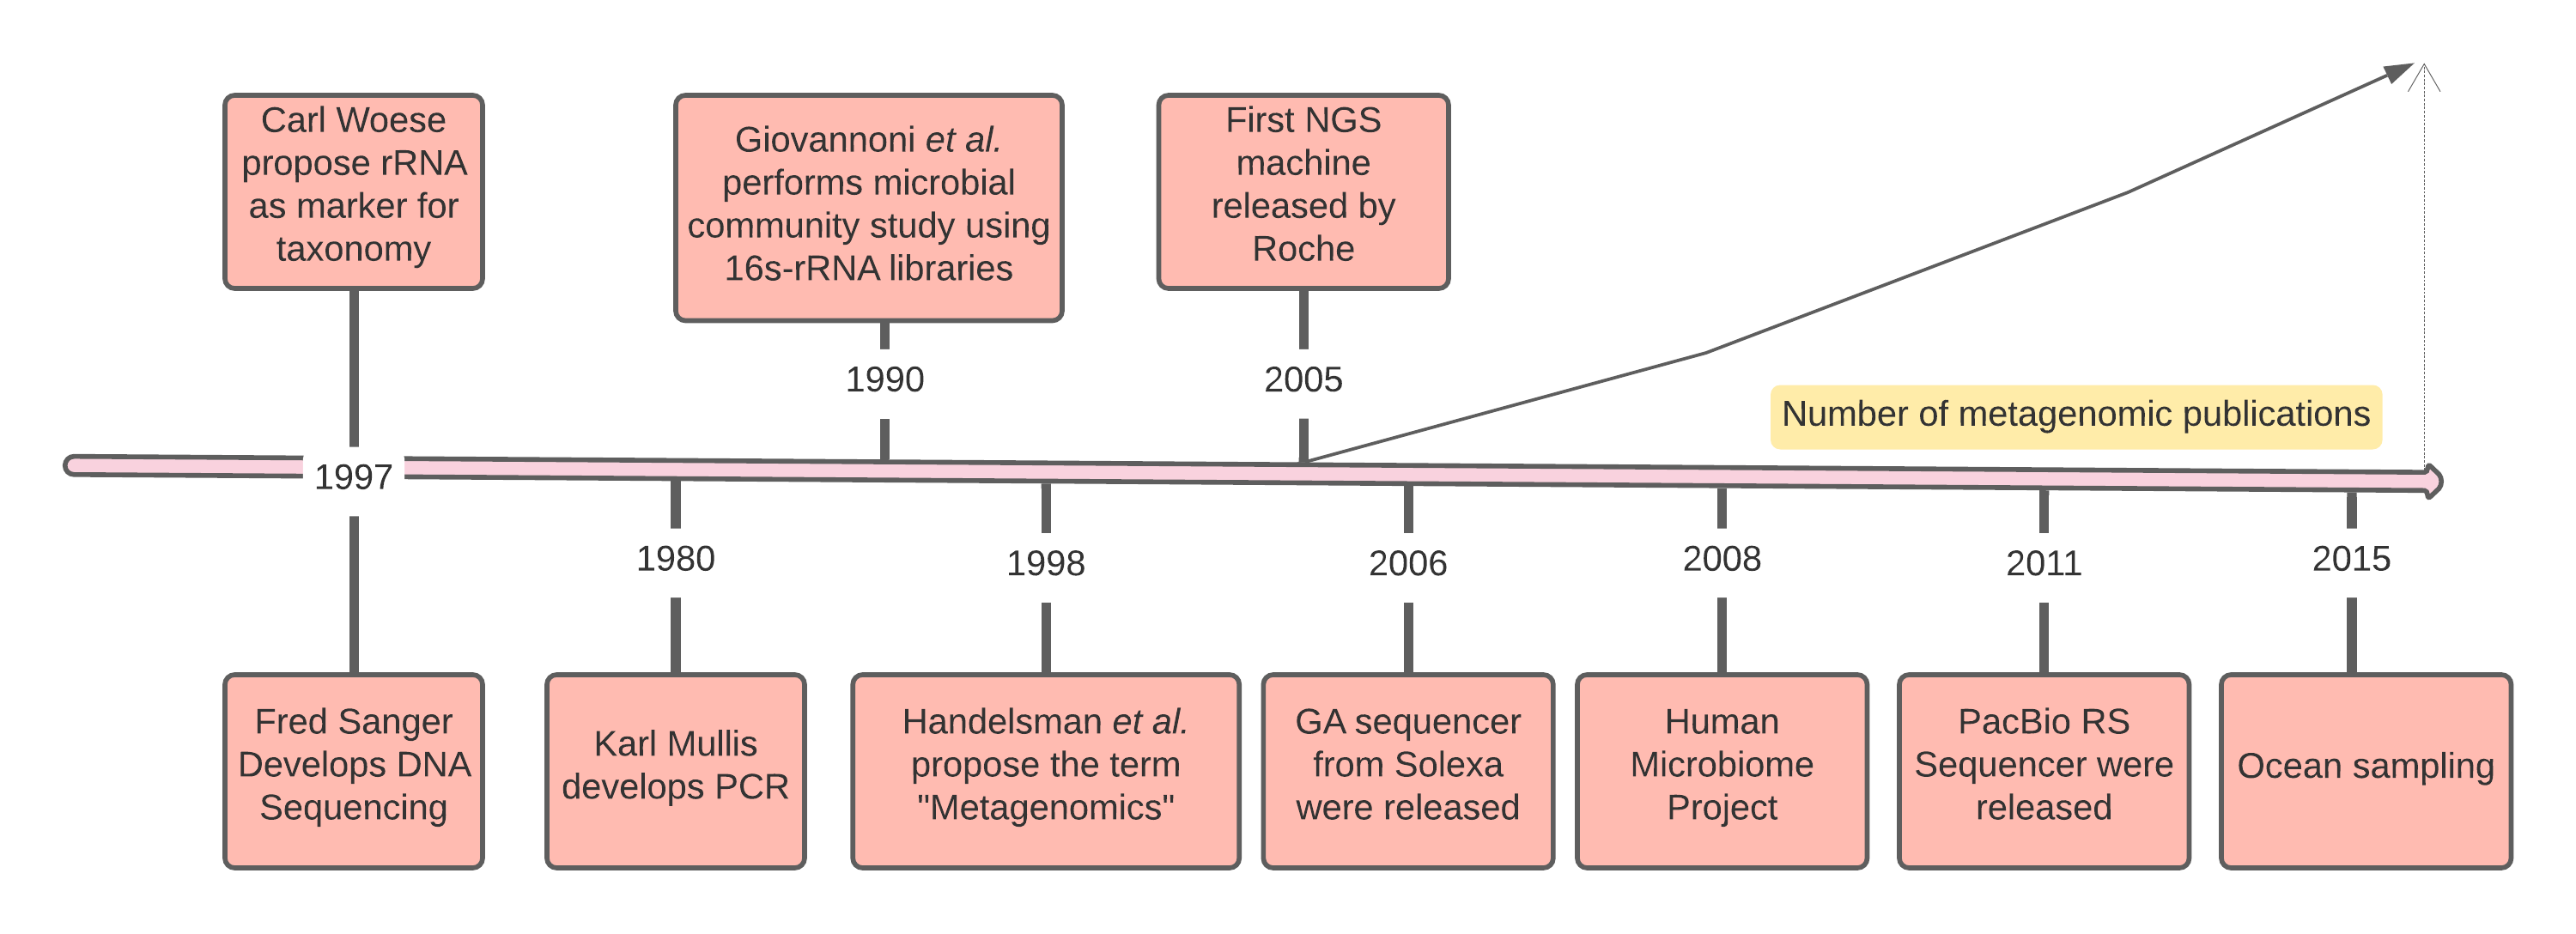
\includegraphics[width=15cm, height=6.5cm]{../figures/Figure2.png}
  \caption[Development of Metagenomics]{Developments in Microbiology with sequencing technology, Infographic displays the rise in the number of publications about metagenomics as the successive generations of sequencers were released starting from 2005 \cite{ref11}}
  \label{fig:figure2}
\end{figure}

Sequence coverage is represented by the average amount of times a nucleotide gets sequenced \cite{ref1}. Therefore, if there is a 10X coverage, then each nucleotide is sequenced ~ ten times. We can measure the expected number reads needed to sequence the whole genome by fitting a Poisson distribution model, which is derived through the Lander-Waterman equation as follows,

\begin{equation} 
  Coverage (C) = \frac{L * N}{G}
  \label{eq:eq1}
\end{equation}

where, L= read length, N = number of reads, and G = length of Genome

\begin{equation} 
  P_{0} = 1 - e^{-C} = P_{0} = 1 - e^{\frac{L * N}{G}}
  \label{eq:eq2}
\end{equation}

\begin{equation} 
  Number  of reads (N) = -\frac{\log(1-P_{0})}{L}* G
  \label{eq:eq3}
\end{equation}

For metagenomic sampling,

\begin{equation} 
  G_{m} = \sum_{i=1}^{\l} n_{i}G_{i}
  \label{eq:eq4}
\end{equation}

Where, $G_{i}$ is size of metagenome containing l genomes; $n_{i}$ is the number of copies of $G_{i}$

\section{Assembly \& Binning}
Assembly of contigs is one of the requisite steps of any genomic data analysis. It allows the researcher to find the genomic elements such as transcription factor binding sites, open reading frames, et cetera. One can also locate notable size elements such as pathogenicity island by assembling longer reads. Like any genomic analysis, the assembly for metagenomics can be done either with a reference dataset or without it (\emph{de-novo} assembly). However, space-time complexity during de-novo assembly increases exponentially; therefore, specially tailored algorithms like de Bruijn are employed for the purpose. And, short-reads should be fabricated in large quantities to procure sufficient coverage. Different read lengths, when assembled, can generate varying information about genetic elements at various levels of complexity [Table \ref{table1}]\cite{ref1}. However, there exist potential challenges when dealing with the metagenomics data, as assembling reads from different OTUs could create interspecies chimaeras.

\begin{table}[ht]
\centering
\caption{Information carried by varying lengths of genomic fragments}
 \begin{tabular}{|c | c|} 
 \hline
 Sequence Length (bp) & Genomic Information \\ [0.5ex] 
 \hline\hline
 25 - 75 & SNPs, Short Frameshift Mutations \\ 
 \hline
 100 - 400 & Short functional signatures \\
 \hline
 500 - 1,000 & Whole domains, Single Domain Genes \\
 \hline
 1,000 - 5,000 & Short Operons, Multi-domain genes \\
 \hline
 5,000 - 10,000 & Long Operons, cis-control elements \\
 \hline
 More than 100,000 & Pathogenicity Islands, Mobile Insertion elements \\
 \hline
 More than 1,000,000 & Prokaryotic Chromosome Organisation \\
 \hline
\end{tabular}
\label{table1}
\end{table}

Binning refers to classifying sheared DNA sequences into taxonomic groups, which describe the individual genomes of the closely related species. Binning can be achieved using two strategies, i.e. either by Composition-based (CB) methods or by Similarity-based (SB) methods. CB binning is prone to errors; as the number and relatedness of OTUs in metagenomes increases, miscalculation frequency also increases \cite{ref11}. Therefore the CB method is preferred for the sequences which have no homologs. Even though the CB method does not yield fruitful results with short reads, the output can be improved by using training datasets of long fragments. SB methods first find the similarities with the available/provided reference dataset to generate a tree and then generate the inferences about the sequences bins. It is clearly a preferred choice of binning method for short reads as it is computationally less intensive to work with smaller contigs.

\section{Functional Annotation}
The functional profile of the metagenome answers vital questions about community dynamics. Ideally, the annotation shouldn't be done de-novo but using a reference dataset. Functional annotation is considerably challenging for traditional genomics data, and complexity further increases when dealing with metagenomes as the available sequences are either partial or have no homologues. The sequences which are not annotated using a reference dataset are known as ORFans and constitute a never-ending genetic recentness in metagenomics \cite{ref12}. To overcome this, one can completely overlook the gene-calling steps and utilize six-frame translation on reads; if the translated frames are adequately long, then they can be considered as ORFs; which can then be used for annotating signatures (HMM profiles etc.). The motif EXtraction (MEX) program works on the same principle and can identify enzymatic elements from sequence data.
\chapter{16s-rRNA Sequencing}
\pagenumbering{arabic} \setcounter{page}{9}

This section presents the science behind 16s-rRNA, how the sequencing is done in order to obtain reads. The section further elaborates on the OTUs and ASVs which are obtained after conducting a bioinformatics analysis. There has been a lot of dispute over the effectiveness of OTUs and ASVs in analyzing the microbial community. Hence, the present section also strives to explain the successes and limitations of both approaches

\subsection{16s ribosomal RNA}
The 16s-rRNA is the RNA part of the 30s small subunit of the ribosome (in prokaryotes).  Inside a prokaryotic cell, it is responsible for scaffolding the position of ribosomal proteins. It also binds to the shine-Dalgarno-Sequence to begin protein synthesis by utilising protein S1 and S21. The 16s-rRNA has seven highly conserved regions flanked by nine hypervariable regions, and therefore it is used in producing phylogenies. The slow rate of evolution 1500 bp long 16s-rRNA makes it a perfect nominee for taxonomic surveys. It is found to be competent in re-classifying prokaryotes into new species and genera. The V4 region is semi-conserved and is proficient in giving phylum-level classification. The V3 region identifies the genus' high accuracy, whereas the V6 is best at distinguishing species. The V1-V8 regions are most effective to include for a disease-specific assay. However, in the families Enterobacteriaceae, Clostridiaceae, and Peptostreptococcaceae, species can have high sequence similarity (99\%); therefore, the V4 sequences can fail to differentiate at lower taxonomic levels. For the taxonomic assignment, there exist highly curated and quality-controlled databases which microbiologists use to assign taxonomies.

\begin{itemize}
  \item \textit{SILVA Database}: It caters an extensive, quality-checked, \& updated datasets of ribosomal sequences for Bacteria, Archaea and Eukarya.
  \item \textit{Ribosomal Database Project (RDP)}: It stores QC passes, aligned and annotated seqs from bactria \& archeas and fungi (28S rRNA).
\end{itemize}

\subsection{16s Amplicon Sequencing}

\begin{enumerate}
  \item \textit{Sampling}: Like any other sequencing, a typical 16s Amplicon sequencing commences with the collection of samples. The samples are directly sourced from the site under study or extracted from the specimen (e.g. gut microbiome).
  \item \textit{Extraction of DNA}: The bulk-DNA is then extracted from the obtained samples using various commercialised preparation kits. The step is very crucial and is often prone to errors due to the presence of environmental DNAse. Therefore, care should be taken during DNA extraction.
  \item \textit{Library Preparation}: The extracted DNA is then sheared and is fragmented into pieces for PCR amplification. This enhances the copy number of the sequence of interest. This step is also prone to technical artefacts, which are somewhat unavoidable. 
  \item \textit{Adaptor Ligation and barcoding}: Adaptors are the known sequences attached along with the 3' and 5' end of the 16-rRNA hypervariable regions (specifically to the V4). The barcodes are added during a multi-plex run which helps in differentiating the samples.
  \item \textit{Sequencing}: Sequencing can be done by a traditional synthesis method, which produces fluorescent signals upon nucleotide addition. Semiconductor based methods like Ion-torrent were initially used however they were discarded as they were error-prone. Technologies like nano-pore, which make long reads, are becoming a standard as they cover the entire length of the 16s-rRNA gene. Nowadays, Illumina sequencing-by-synthesis methodology is used, which, instead of 454 pyrosequencing, produces a lower per-base error and is not susceptive to indels-base errors \cite{ref14}. \textcolor{green}{From a microbial-ecological perspective, the greater throughput of Illumina is the main advantage due to the high diversity of microbial communities.}
  \item \textit{Data Analysis}: The last step involves the data analysis using complex bioinformatics toolkits.This includes the generation of OTUs/ASVs, which can be further used to produce phylogenetic trees and draw conclusions.
\end{enumerate}

\begin{figure}[!hb]
  \centering
  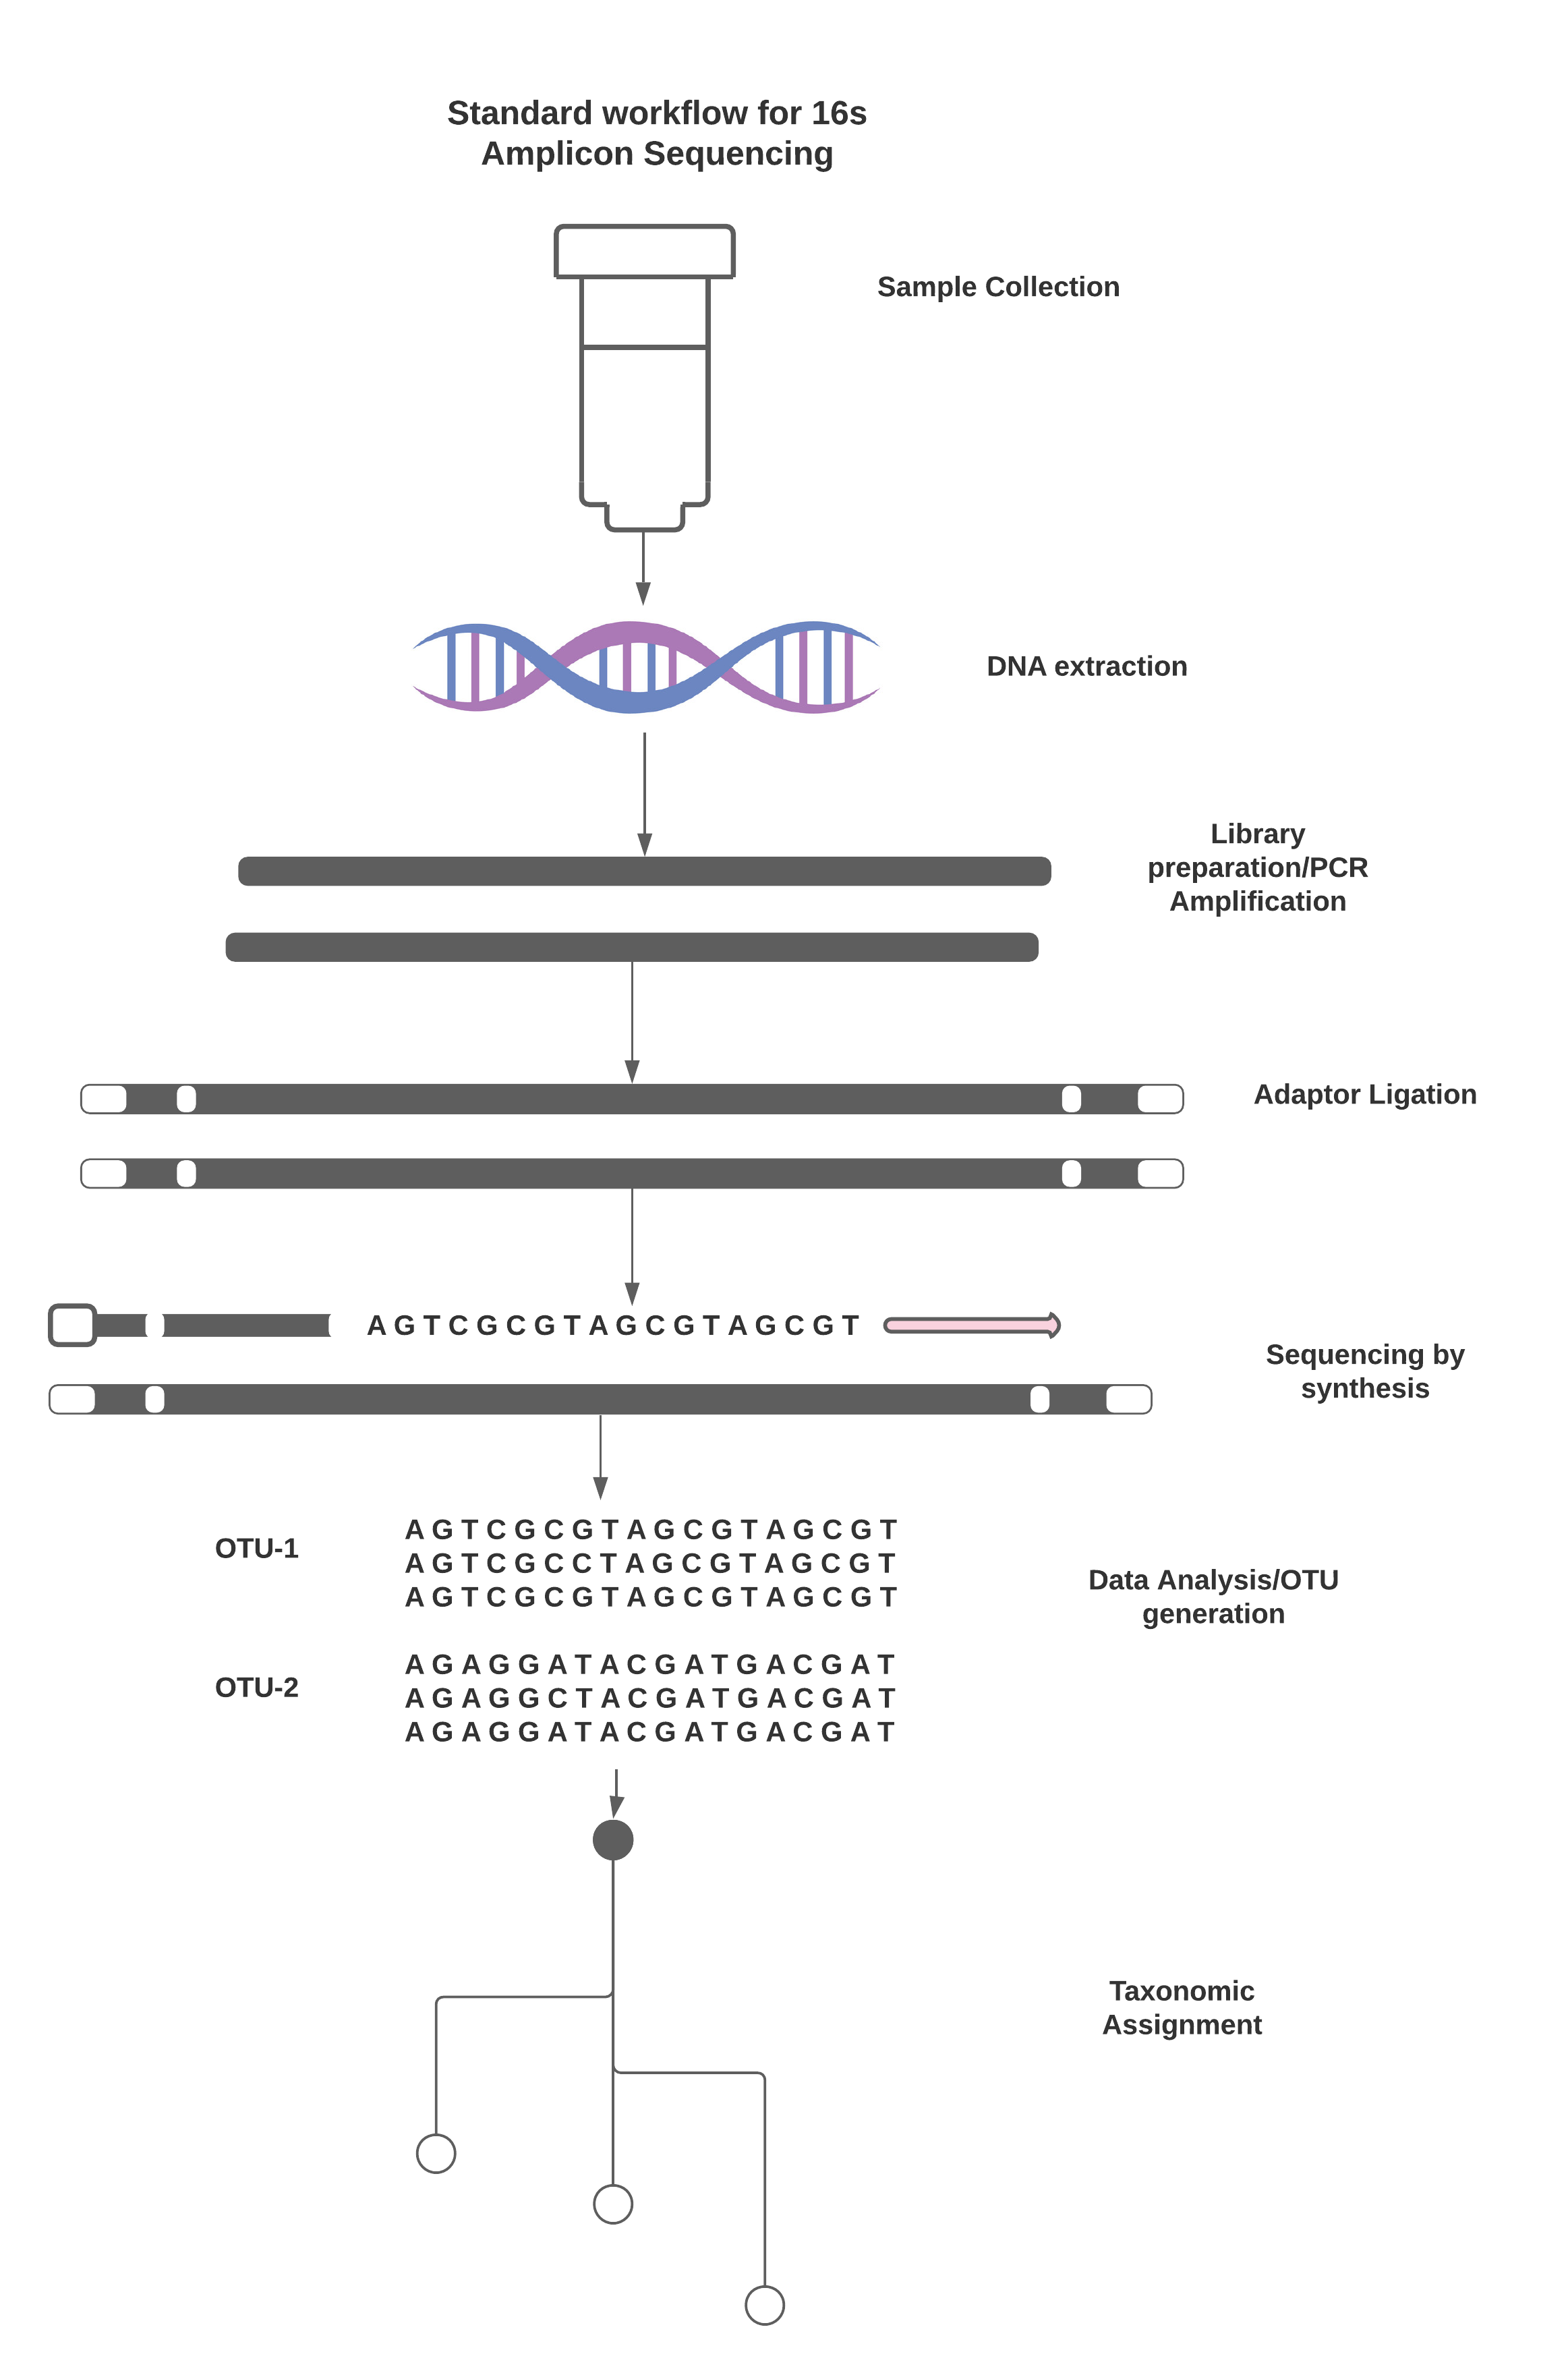
\includegraphics[width=10cm, height=15cm]{../figures/Figure3.png}
  \caption{Standard Workflow for 16s Amplicon Sequencing}
  \label{fig:figure3}
\end{figure}

\subsection{Operational Taxonomic Units}
OTUs are the clusters of sequenced reads that vary by a similarity cut-off. Arguably, the similarity threshold has been set to a constant of 97\% due to many use-cases from 1994. The OTUs thus made are the representatives of a group of sequence reads which are 3\% dissimilar. To be exact, OTUs are pragmatic proxies of the actual sequences read from the data. OTU clusters can either be made using a Hierarchical clustering algorithm such as UCLUST or CD-HIT, or they can be produced using Bayesian clustering approaches such as CROP. However, recent findings have shown that the threshold of 97\% is inefficient to draw ecologically valid conclusions from the data. There has been a dispute about whether the threshold should be tuned depending upon the quality of reads or samples. Even after being a highly questioned concept, the reference-based OTUs are quite accurate compared to de-novo OTUs. OTU clustering can be done with or without using a database. Close reference clustering involves comparing sequences against a curated database, which are then clustered into OTUs \cite{ref15}. However, it suffers if the reference sequence is not present in the dataset. Strengths include the ability to compare OTU assignments across studies. De novo clustering methods calculates the distance between sequences which is then used to cluster sequences into OTUs \cite{ref15}. However, the computational cost scales quadratically with the number of unique sequences. Open-reference clustering also involves performing closed-reference clustering followed by de novo clustering on those sequences that are not sufficiently similar to the reference \cite{ref15}.

\subsection{Amplicon Sequence Variants}
They are also called the Exact Sequence Variants (ESVs) or Zero-Radius OTUs (ZOTUs). They are 100\% non-identical rather than similar and provide a high-resolution picture as opposed to the OTUs as they are resolved down to the difference of one nucleotide \cite{ref16}. Using ASVs, one can detect microbes that may have diverged a million years ago. ASVs from different studies can be mixed if the sequence reads are obtained from a similar genetic locus or if the overlapping regions are trimmed before the merging. Even though ASVs seem to be a sounder option than the OTUs, they have some limitations \cite{ref16}. Firstly, the 16-rRNA gene has more than one copy inside a bacteria, which could vary by 4-base pairs; this will make 4 individual variants into the downstream analysis. Moreover, the complexity of the alpha and beta diversity increase which also further complicates the analysis \cite{ref16}.
\chapter{Pipelines \& Algorithms}
\pagenumbering{arabic} \setcounter{page}{13}

This section examines the two most widely used pipelines that are used to generate OTUs and ASVs. The first pipeline employs the Divisive Amplicon Denoising Algorithm (DADA), which produces the ASVs. The second utilises the Unweighted UniFrac Algorithm (implemented through Mothur), which is used to make OTUs.

\section{DADA}
The DADA is a hierarchical clustering algorithm that works by removing PCR-amplified artefacts from the sequenced reads. The algorithm's goal is to infer the genotypes of the microbes present in the sample along with their error rates. The algorithm operates until the genotypes and errors rates from the noisy sequenced data converge to a mutually consistent set. DADA was compared against the AmpliconNoise algorithm, which it outperformed on various parameters. However, DADA assumes each error to be statistically independent, and there might be a case where a single DNA might produce many artefacts which could induce non-independent errors.\newline

\subsection{Divisive Amplicon Denoising Algorithm}
The p-values ($p_{y}$,$p_{\alpha}$) forms the basis of the algorithms, through which it iteratively updates the partition set of sequence B and the nucleotide error probabilities T. After t iterations the partition set of sequence and the nucleotide error probabilities updates to $B^{t}$ and $T^{t}$. There are three levels of nesting in the algorithm and each of them is repeated until convergence. Beginning with $T^{0}$, the maximum likelihood nucleotide error probabilities are provided partition $B^{0}$ in a unique cluster, and the outermost loop recursively upgrade B \& T until T converges. The following loop begins with the partition, $B^{t}$ = $B^{0}$, and attaches blocks to $B^{t}$ until the $p_{y}$ and $p_{\alpha}$ does not permit rejection of model at common significance levels. If statistically significant families exist that supports both p-values, then a new cluster is formed. After this inner-most loop boosts the probability by reassigning each sequence to the block that would generate the most considerable required amount of reads of that sequence, this proceeds until sequences discontinue renewing clusters.\newline

\begin{figure}
  \centering
  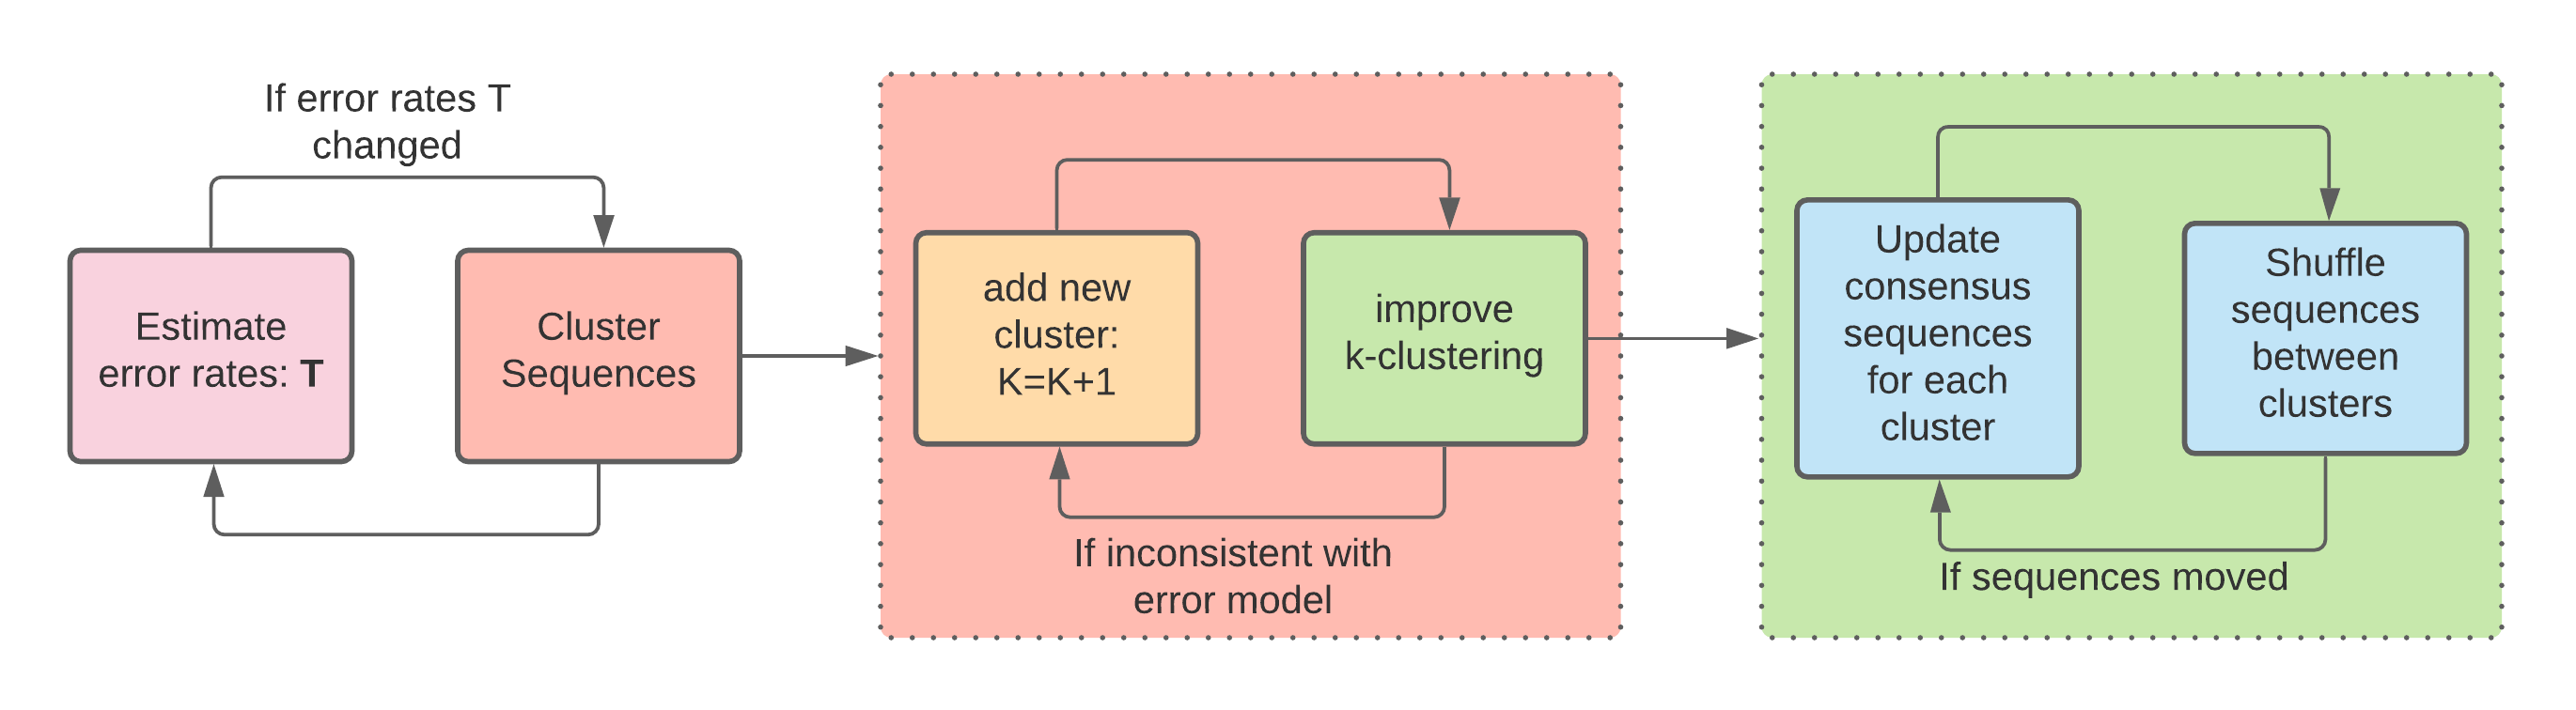
\includegraphics[width=15cm]{../Figure4.png}
  \caption{Schematic representation of DADA algorithm}
  \label{fig:figure4}
\end{figure}

The DADA is currently running in its second version, available as an R library, "DADA2". The DADA2 employ a novel QC-informed model of Illumina amplicon errors. The DADA2 pipeline commences with the command "fastqFilter()", which trims adaptors, removes short sequences and ambiguous bases. DADA can apply this to both paired-end and single-end reads. This step is accompanied by the "derep()" function, which performs the dereplication of the data. Lastly, the DADA's de-ionising algorithm is implemented, which is explained in  \ref{fig:figure4}; it estimates genotypes and calculates errors. One can also remove chimaeras by performing Needleman-Wunsch global alignment using the function "isBimeraDenovo()". The complete pipeline of DADA2 is given in Appendix-1.

\section{MOTHUR}
The MOTHUR is a comprehensive tool written in C++ using Object-Oriented-Programming (OOPs) fundamentals. It integrates the algorithms from previous packages/tools, including SONS, DOTUR, and TreeClimber. MOTHUR operates on various clustering algorithms such as the nearest neighbour, OptiCLust, Unweighted-pair group method using average linkages (UPGMA). Here I discuss the OptiCLust algorithm, which is the default algorithm of MOTHUR that produces OTUs.

\subsection{OptiClust}

\begin{figure}[!hb]
  \centering
  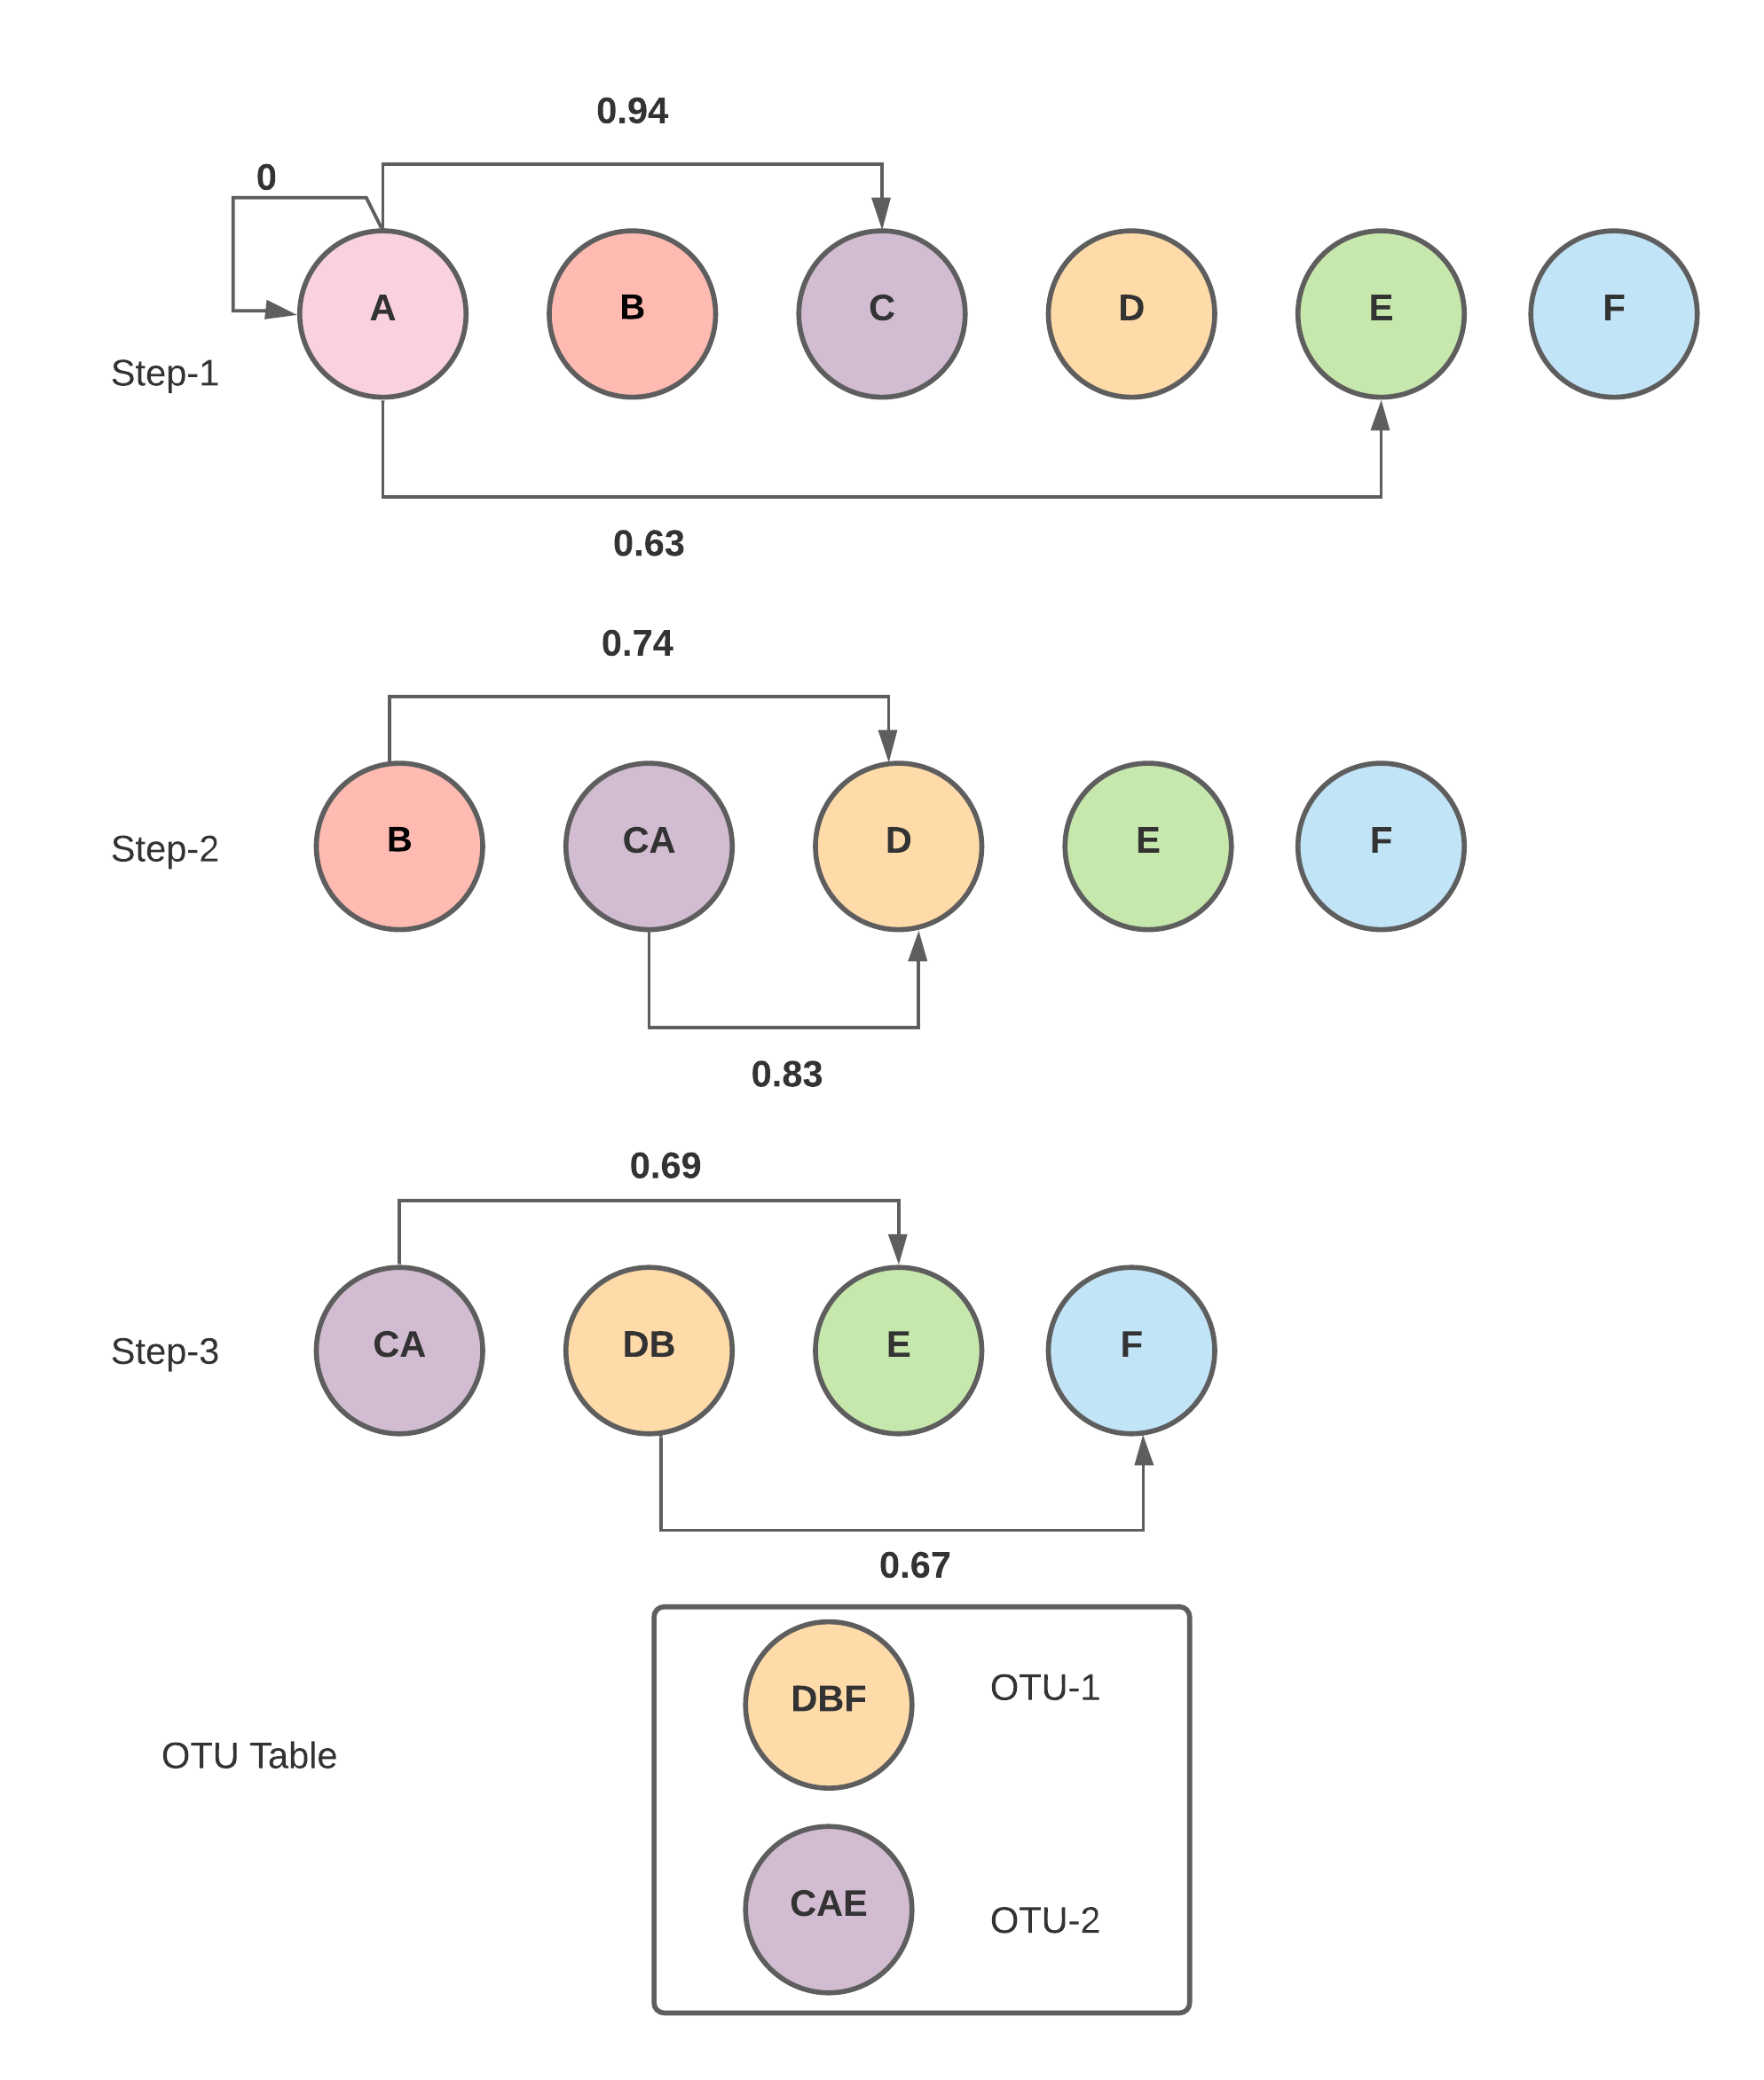
\includegraphics[width=10cm, height=12cm]{../Figure5.png}
  \caption{Schematic representation of OptiClust algorithm}
  \label{fig:figure5}
\end{figure}

The OptiCLust begins by calculating the pairwise distance between all the sequences. It then removes the sequences having a pairwise distance less than a threshold. Once the filtered set is obtained, it seeds by assigning each sequence a distinct OTU. The convergence initiates by calculating Matthew's Correlation Coefficient (MCC) between the first singleton OTU and the other sequences. The MCC for singleton OTU itself is zero; therefore, it chooses the different available sequences that increase the MCC value. If the change in the MCC is the same between the two sequences then, it randomly selected either of the two. This step is repeated until the entire sequence set is converted into OTUs [Figure \ref{fig:figure5}]. To initiate OptiClust algorithm requires either a phylip-formatted distance matrix or a column-formatted distance matrix. The "cluster" command initiates the clustering process that creates the OTUs.
\chapter{Phylogenetic Measures}
\pagenumbering{arabic} \setcounter{page}{16}

\textcolor{red}{This section discusses the four most widely used approaches that are used in designing the phylogenetic trees. The approaches are classified distance based-approaches and character-based approaches.}

\subsection{Distance-based approaches}

\textcolor{red}{As the name suggests, the distance-based algorithms utilise the matrices containing pairwise distances. Pairwise distances aid in the construction of trees via Bayesian and likelihood methods. The two most widely used methods which utilise the pairwise distance are the Unweighted Pair Group Method with Arithmetic Mean (UPGMA) and Neighbour Joining (NJ) method \cite{munjal_2019_phylogenetics}. UPGMA is an agglomerative hierarchical clustering method that builds a rooted phylogenetic tree by assuming equal rates of evolution. The NJ is an iterative clustering method that produces an unrooted tree by considering different rates of evolution. Given that both the methods use a distance matrix, they lower computing time for large datasets compared to character-based methods. NJ is preferred over UPGMA for almost all cases as the previous assumes the same evolution rate for all of its lineages \cite{munjal_2019_phylogenetics}.}

\subsection{Character-based approaches}

\textcolor{red}{The character-based approaches use actual sequence alignments similarities to calculate the distances. The character-based methods are more greedy for computational resources and time as compared to the distance-based techniques \cite{munjal_2019_phylogenetics}. However, they generate exact phylogenetic trees. The character-based methods include Maximum-Likelihood (ML) and Maximum-Parsimony (MP). The MP is based on the assumption that the simplicity extends that the most parsimonious tree would be the one that reflects the slightest evolutionary changes \cite{munjal_2019_phylogenetics}. The ML, on the other hand, utilises the probabilistic modelling based on Markov chains to derive the trees.}

\subsection{Bootstrapping}

\textcolor{red}{Once the trees are constructed, the inference of their reliability poses a challenge. This is known as bootstrapping. Bootstrapping in phylogenetic analysis is a greedy approach that picks deviated/pseudo samples from the original dataset to design the tree \cite{lemoine_2018_renewing}. Essentially, running any tree constructing algorithms on a sample data more than 100 times generates a bootstrapping value which is a measure of reliability as it gives the probability of a branch.}

\subsection{Microbial Community \& Phylogeny}

\textcolor{red}{Bacterial lineages determine how the microbial communities are formed as the phylogenetic relatedness points towards functional relatedness. Traits of bacteria influencing ecological functions are phylogenetically conserved. High ecosystem functioning is directly related to the co-existence of functionally distinct lineages or from the existence of productive lineages that outperform the rest. Functional differences allow coexistence through niche segregation events and deliver different functions to the ecosystem. A study performed by \emph{Goberna et al} detected that the abundance of divergent lineages in the community increases the ecological processes \cite{goberna_2018_phylogeneticscale}. Therefore to elucidate the ecological functioning of the community, incorporation of phylogenetic measures is very crucial.}
\chapter{Co-occurrence Networks}
\pagenumbering{arabic} \setcounter{page}{18}

The microbes do not dwell in isolation; instead, they thrive in colonies and form associations. These associations shape the patterns and structure of their microscopic world, which administers the macroscopic world. For example, the gut microbiome regulates the food choices of an individual. The interaction patterns among these microbes are directed by their evolutionary cycle and inter/intra-species interactions. They can have a positive association like mutualism, commensalism, synergism, or negative associations like competition, parasitism, predation \cite{weiss_2016_correlation}. To analyse these associative patterns, microbiologists have implemented the concepts of networks science onto these associations. The graphical form of these pairwise associations is called a microbial co-occurrence network. The nodes of the networks denote the microbial species, and the edges of the network describe the statistically significant association. These co-occurrence networks also help determine the critical microbial species or hubs dominating a particular community.\newline

However, drawing adequate ecological conclusions from an entirely mathematical concept is not advisable. Criticisms have been made about co-occurrence networks for predicting non-trophic interactions, which calls for integrating community-level insights. Studies have shown that processes like habitat filtering should be considered while generating the co-occurrence networks to draw ecologically sound conclusions. \emph{Goberna et al} have compared the effect of habitat filtering, spatial limitation, and biological interactions in governing the community patterns; the study found that habitat filtering and natural interactions are much more predominant than dispersal limitations \cite{ref10}. This might suggest that associations form independent of their geographical location. They also explained the need to consolidate phylogenetic measure into the downstream analysis to make the networks a close imitation of nature. One might overshadow that the microbes can interact with more than one neighbour, which gives triplet or quadrupole interactions, rather than a pairwise interaction \cite{berry_2014_deciphering}. This section discusses widely used measures in co-occurrence networks design, such as Pearson correlation, Spearman Correlation and Bray-Curtis similarity measure.

\section{Pearson's Correlation}
The Pearson's Correlation (PC) estimates the magnitude of the linear covariance between two independent variables \cite{schober_2018_correlation}. The data should be randomly sampled and devoid of outliers showing linear patterns in a scatter-visual test. It assumes that data follows normal distribution the values of a variable are not correlated to themselves \cite{schober_2018_correlation}. The test works with continuous data points sampled or for a paired observation. In terms of co-occurrence networks, the microbial pair forms an {x,y} set of statements, given that there is no correlation between $x_{i}$ or $x_{n}$/$y_{i}$ or $y_{n}$, where (i = 1). Pearson's correlation calculates three measures, i.e. Coefficient (r), Coefficient of determination ($R^{2}$), and p-value. The r tells the direction and strength to which the x and y are correlated. The r can range between (-1,1), with -1 suggestive of a strong negative correlation and 1 suggestive of a strong positive correlation. The $R^{2}$ explains the variation shared between the x and y, and it can range between (0,1). Lastly, the p-value measures the evidence against the null hypothesis ($H_{0}$) that there is no correlation between x and y. The working formula boils down to dividing the covariance by the product of the standard deviations,

$$r_{xy} = \frac{\sum_{i=1}^{n} (X_{i} - \bar{X}) * (Y_{i} - \bar{Y})}{\sqrt{\sum_{i=1}^{n} (X_{i} - \bar{X})^{2}} * \sqrt{\sum_{i=1}^{n} (Y_{i} - \bar{Y})^{2}}}$$

\section{Spearman's Correlation}
The Spearman's Correlation (SC) estimates magnitude \& direction of the monotonic relation among the two ranked variables \cite{dewinter_2016_comparing}. The SC is implemented on the ordinal data rather than continuous data. It assumes a monotonic association between the variables, i.e. if one is changing, the other remains the same. The SC is well suited for explaining interactions like amensalism. It does not assume the data to be normally distributed and works by ranking the variables first. As the variables are ranked according to their magnitude, they can be implemented on both ordinal and continuous datasets. Pearson's correlation calculates three measures, i.e. Coefficient ($r_{s}$) and p-value. The rs tells the direction and strength to which the x and y are correlated. The $r_{s}$ can range between (-1,1), with -1 suggestive of a perfect negative correlation and 1 suggestive of a perfect positive correlation \cite{dewinter_2016_comparing}. Lastly, the p-value measures the evidence against the null hypothesis ($H_{0}$) that there is no correlation between x and y. The working formula boils down to dividing the Pearson correlation over the (mean) ranks,

$$r_{s} = 1 - \frac{6 * \sum D^{2}}{n^{3} - n}$$

\section{Bray Curtis Dissimilarity}
The Bray Curtis Dissimilarity (BC) quantifies the dissimilarity between the species between two different sites. In terms of microbial ecology, one can say it measures the beta-diversity by comparing the alpha-diversity \cite{zhang_2019_the}. It falls between 0 to 1, with 0 suggesting that they are identical, and one is suggestive of 100 per cent dissimilar. The BC dissimilarity assumes that both the sampling sites have either the same size or same volume as the BC does not integrate the notion of space \cite{zhang_2019_the}. The BC can be calculated by dividing the sum of lesser counts of species found in both sites by the sum of the alpha-diversity measure of each site,

$$BC_{ij} = 1 - \frac{2 * C_{ij}}{S_{i} + S_{j}}$$


%Included for Gather Purpose only:
\addcontentsline{toc}{chapter}{Bibliography}
\bibliographystyle{ieeetr}
\bibliography{mybibliography}

\addcontentsline{toc}{chapter}{Appendices}
\chapter*{Appendix}

\pagenumbering{arabic} \setcounter{page}{21}

\subsection*{DADA2 Pipeline}
The follwoing pipeline is written in R version 4.0.5 (2021-03-31)

\subsubsection*{Syntax for loading libraries}

\begin{lstlisting}[language=R]
# Required Libraries
library(dada2) # Version 1.18.0
library(ggplot2) # Version 3.3.3
library(DECIPHER) # Version 2.18.1
library(phangorn) # Version 2.5.5
library(phyloseq) # Version 1.34.0
\end{lstlisting}

\subsubsection*{Syntax for setting filepaths and conventions}

\begin{lstlisting}[language=R]
# Reading path for untrimmed fastq files
untrimmed <- file.path("fastqFiles/")

# Sorting the filenames
fns <- sort(list.files(untrimmed, full.names = TRUE))

# Roots for forward reads
fnFs <- fns[grepl("_R1", fns)]

# Roots for reverse reads
fnRs <- fns[grepl("_R2", fns)]

# Directory for filtered output (Removal of Ns)
filtFs <- file.path("filtered",fnFs) # Forward
filtRs <- file.path("filtered",fnRs) # Reverse

names(filtFs) <- fnFs # Forward
names(filtRs) <- fnRs # Reverse
\end{lstlisting}

\subsubsection*{Syntax for quality control (QC-Trim)}

\begin{lstlisting}[language=R]
out <- filterAndTrim(fwd = fnFs, # Roots for forward reads
  filt = filtFs, # Path for filtered forward reads
  rev = fnRs, # Roots for reverse reads
  filt.rev = filtRs, # Path for filtered reverse reads
  maxN = 0, # Removing Ns
  maxEE = c(2,2),
  truncQ = 0, truncLen = 245, # Trimming start/stop
  rm.phix=FALSE, multithread=TRUE,
  compress = T)
\end{lstlisting}

\subsubsection*{Syntax for dereplicating}

\begin{lstlisting}[language=R]
derepFs <- derepFastq(filtFs)
derepRs <- derepFastq(filtRs)
sam.names<-sapply(strsplit(basename(filtFs),"_"),'[', 1)
names(derepFs) <- sam.names
names(derepRs) <- sam.names
\end{lstlisting}

\subsubsection*{Syntax for error model estimation}

\begin{lstlisting}[language=R]
# Forward
ddF <- dada(derepFs[1:10], err=NULL, selfConsist=TRUE)

# Reverse
ddR <- dada(derepRs[1:10], err=NULL, selfConsist=TRUE)
\end{lstlisting}

\subsubsection*{Syntax for running DADA}

\begin{lstlisting}[language=R]
# Forward
dadaFs <- dada(derepFs, err=ddF[[1]]$err_out, pool=TRUE)

# Reverse
dadaRs <- dada(derepRs, err=ddR[[1]]$err_out, pool=TRUE)
\end{lstlisting}

\subsubsection*{Syntax for Merging and Extracting ASV}

\begin{lstlisting}[language=R]
# Merging forwards and Backward reads
mergers <- mergePairs(dadaFs, derepFs, dadaRs, derepRs)

# Extracting Seqs
seqtab.all <- makeSequenceTable(mergers)

# Removing Chimeras
seqtab <- removeBimeraDenovo(seqtab.all)
\end{lstlisting}

\subsubsection*{Syntax for Assigning Taxonomy with RDP taxonomic training data 
formatted for DADA2 (RDP trainset 16/release 11.5)}

\begin{lstlisting}[language=R]
# Using assignTaxonomy() from dada2
asv_rdp_tax <- assignTaxonomy(seqtab,
"trainingSets/rdp_train_set_16.fa.gz , multithread=TRUE)
\end{lstlisting}

\subsection*{\newline MOTHUR Pipeline}
The follwoing pipeline is from MOTHUR Version 1.35.1

\subsubsection*{Syntax for making contigs}

\begin{lstlisting}[language=R]
make.contigs(file=stability.files, processors=8)
\end{lstlisting}

\subsubsection*{Syntax for trimming}

\begin{lstlisting}[language=R]
screen.seqs(fasta,groups,maxambig=0,maxlength=275)
\end{lstlisting}

\subsubsection*{Syntax for trimming}

\begin{lstlisting}[language=R]
screen.seqs(trim.fasta,stability.groups,maxlength=275)
\end{lstlisting}

\subsubsection*{Syntax for dereplication}

\begin{lstlisting}[language=R]
unique.seqs(fasta=stability.trim.contigs.good.fasta)
\end{lstlisting}

\subsubsection*{Syntax for taxanomic Assignment}

\begin{lstlisting}[language=R]
align.seqs(fasta=unique.fasta,reference=silva.v4.fasta)
\end{lstlisting}


\subsubsection*{Syntax for OTU clustering}

\begin{lstlisting}[language=R]
pre.cluster(unique.fasta,otu_table,diffs=2)
\end{lstlisting}

\subsubsection*{Syntax for Counting OTUs}

\begin{lstlisting}[language=R]
chimera.vsearch(cluster.fq,otu_table,dereplicate=t)
\end{lstlisting}

\subsubsection*{Syntax for removing chimeras}

\begin{lstlisting}[language=R]
remove.seqs(fasta=precluster.fq,accnos=denovo.fq)
\end{lstlisting}

\end{document}
